\documentclass[12pt]{report}

\usepackage[a4paper]{geometry}
%\geometry{left=2.5cm,right=2.5cm,top=2.5cm,bottom=2.5cm, a4paper}
\usepackage[utf8]{inputenc}
\usepackage{amsmath}
\usepackage{amsthm}
\usepackage{amssymb}
\usepackage{ulem}
\usepackage{graphicx}
\usepackage{caption}
\graphicspath{}
\usepackage[document]{ragged2e}
\usepackage{setspace}
\usepackage{tabularx}
\usepackage[slovene]{babel}
\usepackage{gensymb}
\usepackage{siunitx}
\usepackage{pdfrender,xcolor}
\usepackage{hyperref}
\usepackage{xurl}
\usepackage{float}
\usepackage{titlesec}

\newfloat{slika}{htbp}{loc}
\floatname{slika}{Slika}

\newfloat{tabela}{htbp}{loc}
\floatname{tabela}{Tabela}

\title{
  
\includegraphics[width=0.4\textwidth]{fmf_logo}\\
  {\small Oddelek za fiziko} \\
  {Feromagnetizem}\\
  {\small Poročilo pri fizikalnem praktikumu III}\\

}
\date{2022/23}
\author{ Kristofer Čepon Povšič \\[5 cm]
 \small  Mentor: Jelena Vesić
}


\titleformat{\chapter}[hang]{\Huge\bfseries}{\thechapter{. }}{0pt}{\Huge\bfseries}

\setlength\parindent{0pt}

\begin{document}

\setcounter{page}{2}

\maketitle

\chapter*{Uvod}

Mnogi električne spoijine in zlitine so feromagnetne. Njihova magnetna permeabilnost $\mu$ je $\gg 1$, vendar ni konstantna in odvisna od jakosti magnetnega polja H. Zveza med gostoto magnetnega polja in njegovo jakostjo je nelinearna in se jo zapiše z enačbo: 

\begin{equation}
  \mu = \frac{1}{\mu_0}\frac{dB}{dH}
\end{equation}

kjer je $\mu_0$ indukcijska konstanta. Zgornji diferencialni kvocient tvori grafično magnetilno in histerezno krivuljo. Iz krivulj lahko spoznamo pomembne lastnosti o snovi. 

Feromagnetna snov je magnetizirana, ko ni v zunanjem polju. Magnetizacija je posledica urejenih magnetnih ionov v feromagnetni snovi. 

V makroskopskem kosu feromagnetne materije so redko vsi magnetni momenti razporejeni vzporedno in tvorijo magnetno polje. V njej se tako pojavijo domene s svojo magnetizacijo. Energija magnetnega polja je najmanjša, če se sklene magnetni pretok znotraj snovi. 

V feromagnetu, ki je v magnetnem polju, se domene, ki kažejo v podobno smer kot magnetno polje povečajo, ostale pa ne. Za dovolj veliko magnetni polje se vse magnetne domene preuredijo, da kažejo vzporedno. 

Odvisnost B(H) je pri manjšanju magnetne jakosti drugačna kot pri večanju - histereza. Pri $H=0$ je $B \geq 0$. $B_R$ pri $H_0$ rečemo remanentna gostota magnetnega polja. 

Imamo feromagnetno jedro s konstantnim presekom in majhno režo s površino S navito v tuljavi z n ovoji, po kateri teče tok I. Velja: 

\begin{equation}
  U_m = \oint \vec{H} \,d\vec{s} = \sum I = n I
\end{equation}

Za naš primer velja: 

\begin{equation}
  U_m = U_{fero} + U_{reza} = LH_{fero} + xH_{reza} = Njihova
\end{equation}

kjer je $L$ dolžina feromagneta in $x$ širina reže. 

Magnetni pretok $\phi_m$ je:

\begin{equation}
  \phi_m = SB_{fero} = SB_{reza}
\end{equation}

Iz magnetnega pretoka vidimo, da je jakost magnetnega polja v reži in feromagnetu enaka. V reži pa velja zveza $B_{reza} = \mu_0 H_{reza}$. Pri $I = 0$, $H_{fera}\text{, } H_{reza} \geq 0$, dobio zvezo: 

\begin{equation}
  H_{reza} = -\frac{L}{x} H_{fero} 
\end{equation}

Upoštevajoč enakost jakosti magnetnega polja dobimo enačbo: 

\begin{equation}
  B_{fero} = - \mu_0 \frac{L}{x} H_{fero}
\end{equation}

\chapter*{Naloga}

\begin{enumerate}
  \item Izmeri histerezno zanko transformatorskega jekla
  \item Določi vrednosti gostote magnetnega polja v reži magnetnega kroga sestavljenega iz transformatorskega jekla kot funkcijo debeline reže in toka napajanja. Primerjaj izmerjeni rezultat $B_{reza}$ pri I = 0 z vrednostjo, ki jo določiš iz prej izmerjene histerezne krivulje. 
  \item Izmeri histerezno krivuljo za magnetni krog sestavljen iz dveh delov. Prvi del je transformatorsko jeklo, drugi del je masivni kos železa. Dodatno: Izračunaj histerezno krivuljo kosa masivnega železa. 
\end{enumerate}


\begingroup
\let\clearpage\relax

\chapter*{Potrebščine}
\begin{itemize}
  \item transformatorski krog(jarem), zaključek magnetnega kroga iz transformatorskega jekla in železa
  \item distančniki 
  \item primarna tuljava ($N_1 = 1000$) in sekundarna tuljava ($N_2 = 46$)
  \item elektronsko procesno vezje v škatli, ki je povezano preko USB povezave z računalnikom 
\end{itemize}

\chapter*{Navodilo}

Magnetni krog zaključimo s kosom transformatorskega jekla ali železa, z distančniki pa izbiramo širino reže. Najprej nariši histerezno krivuljo transformatorskega jekla. Za različne debeline reže nariši histerezne krivulje in odčitaj vrednost gostote magnetnega polja pri $U_m=0$. Izriši še histerezno krivuljo za magnetni krog sestavljen iz dveh delov, ki vsebuje kos masivnega železa. 
\endgroup


\chapter*{Obdelava podatkov}

\section*{Histerezna krivulja jekla}

Površino sestavlja kvadratna ploskev s stranico $a = 4cm \pm 0.5cm$. Za obseg vzamem povprečje zunanje in notranjega obsega in dobim stranici $b = 10.6cm \pm 0.4cm$ in $c = 13.3cm \pm 0.4cm$. 

Na vodoravno os nanesem magnetno jakost $H = \frac{NI}{L}$, kjer je $L = 2a + 2b$ in $N=1000$ ovojev primarne tuljave. Na navpično os nanesem magnetno gostoto $B= \frac{F}{SN_2} - B_0$, kjer je $F$ zajeta iz integrala in S presek kroga, $N_2 = 46$ število navojev sekundarne tuljave in $B_0$ polovica razlike najmanjše in največje dosežene gostote. 

Dobimo krivuljo na grafu \ref{fig:hisJ}. 

\begin{slika}[H]
  \centering
  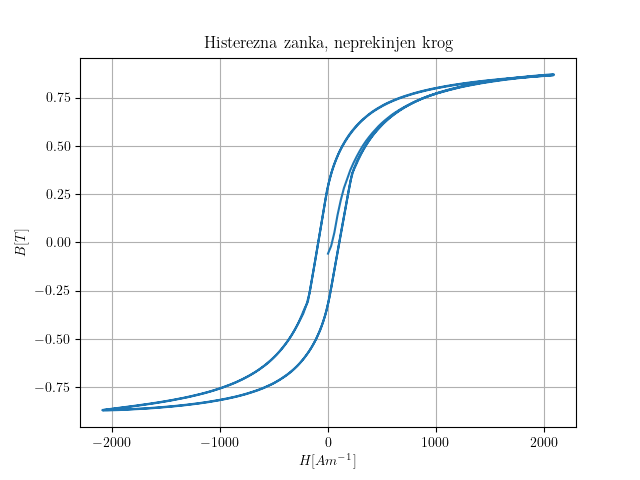
\includegraphics[width=0.75\textwidth]{jeklo}
  \caption{\small Graf prikazuje histerezo neprekinjenega kosa jekla.}
  \label{fig:hisJ}
\end{slika}

\section*{B v odvisnosti od debeline reže}

Na isti način kakor prej narišem histerezo za debeline rež od 3 do 18 listkov. Ne poznam dejanske vrednosti H, zato na vodoravno os nanašam $U_m =N I$. Krivulje so prikazane na sliki \ref{fig:hisR}.

\begin{slika}[H]
  \centering
  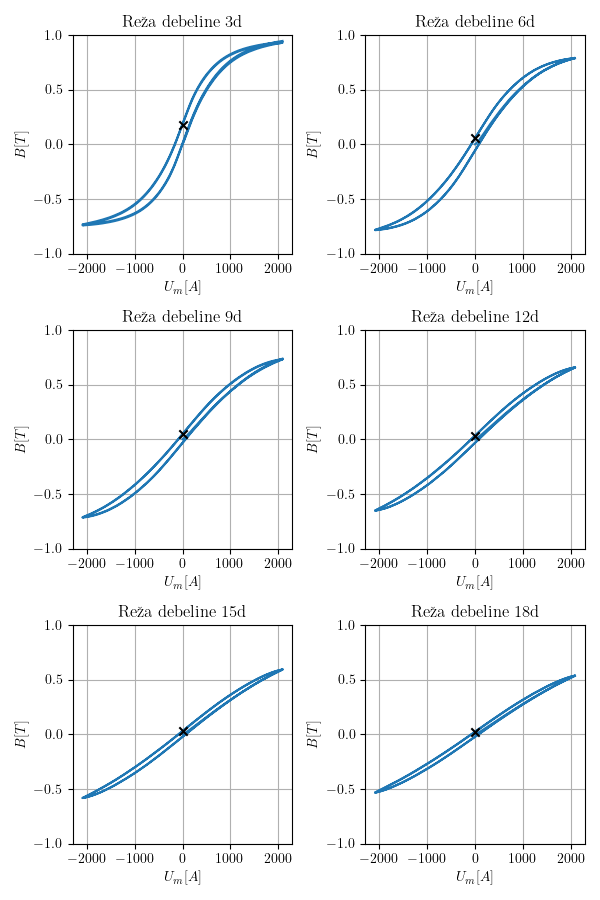
\includegraphics{grafi}
  \caption{\small Histerezne krivulje pri različnih debelinah rež}
  \label{fig:hisR}
\end{slika}

Remanentne gostote v krogu z režo lahko dobimo kot gostoto v presečiščih krivulj s premico $U_m = 0$. Te vrednosti lahko tudi izračunam po enačbi: 

\begin{equation}
  B = -\mu_0 \frac{L}{d}H
\end{equation}

kjer je L notranji obseg kroga in d mnogokratnik debeline lističa. Izračunane in izmerjene vrednosti so prikazane v tabeli: 

\begin{tabela}[H]
  \centering
  \begin{tabular}{|c|c c|c c|} \hline
    $\frac{d}{d_0}$ & $B_{rac}$ & $B_{izm}$ & $\delta B$ & $\sigma B$ \\ \hline
    3 & 118.4 & 179.3 & 60.8 & 0.5 \\ \hline
    6 & 73.6 & 55.4 & 18.2 & 0.2 \\ \hline
    9 & 53.4 & 45.0 & 8.4 & 0.2 \\ \hline
    12 & 41.9 & 33.3 & 8.6 & 0.2 \\ \hline
    15 & 34.5 & 28.5 & 6.0 & 0.2 \\ \hline
    18 & 29.3 & 23.0 & 6.3 & 0.2 \\ \hline
  \end{tabular}
\end{tabela}

\section*{Histereza masivnega kosa železa}

Ponovno narišem histerezo, kjer na vodoravni osi ponovno uporabimo $U_m$. 

\begin{slika}[H]
  \centering
  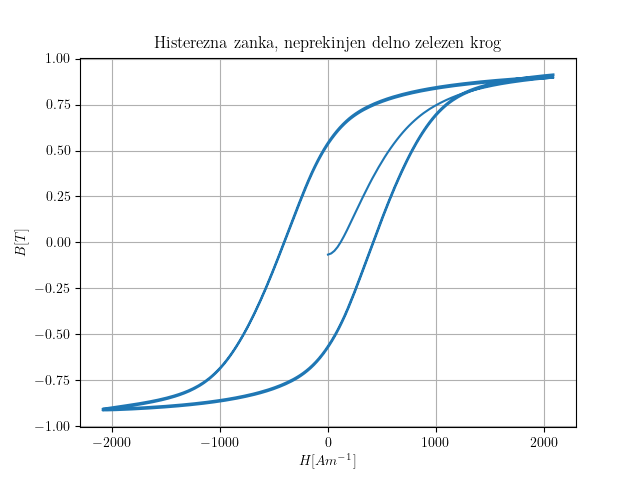
\includegraphics[width=0.75\textwidth]{zelezo}
  \caption{\small Graf prikazuje histerezo masivnega kosa železa in transformatorskega kroga.}
\end{slika}

Železni del kroga ima dolžino $l$, torej ima del iz transformatorskega jekla z dolžino $L-l$. Po Amperovem zakonu izrazimo vrednost, ki jo želimo izračunati

\begin{equation}
  H_{Fe} = \frac{1}{l} \left(NI - (L - l)H_j\right)
\end{equation}

Iz meritve delno železnega kroga poznamo v točki gostoto v železu B in tok skozi primarno tuljavo I. Ker je poleg tega magnetna gostota v jeklu in v železu enaka (krog ima konstanten presek), lahko iz meritve neprekinjenega kroga iz transformatorskega jekla za določeno gostoto B (v železu in jeklu), določimo magnetno jakost v jeklu $H_j$. 



\end{document}